
%------------------------------------------------------------------------
\begin{frame}
	\frametitle{Derivation in Scotto's \emph{Tetralogy}}
	Let $S = \{ 0, 4, 7, 3, 11, 2, 10, 1, 6, 8, 9, 5 \}$ and consider the self-derivation array below.
    \begin{figure}
    	\centering
    	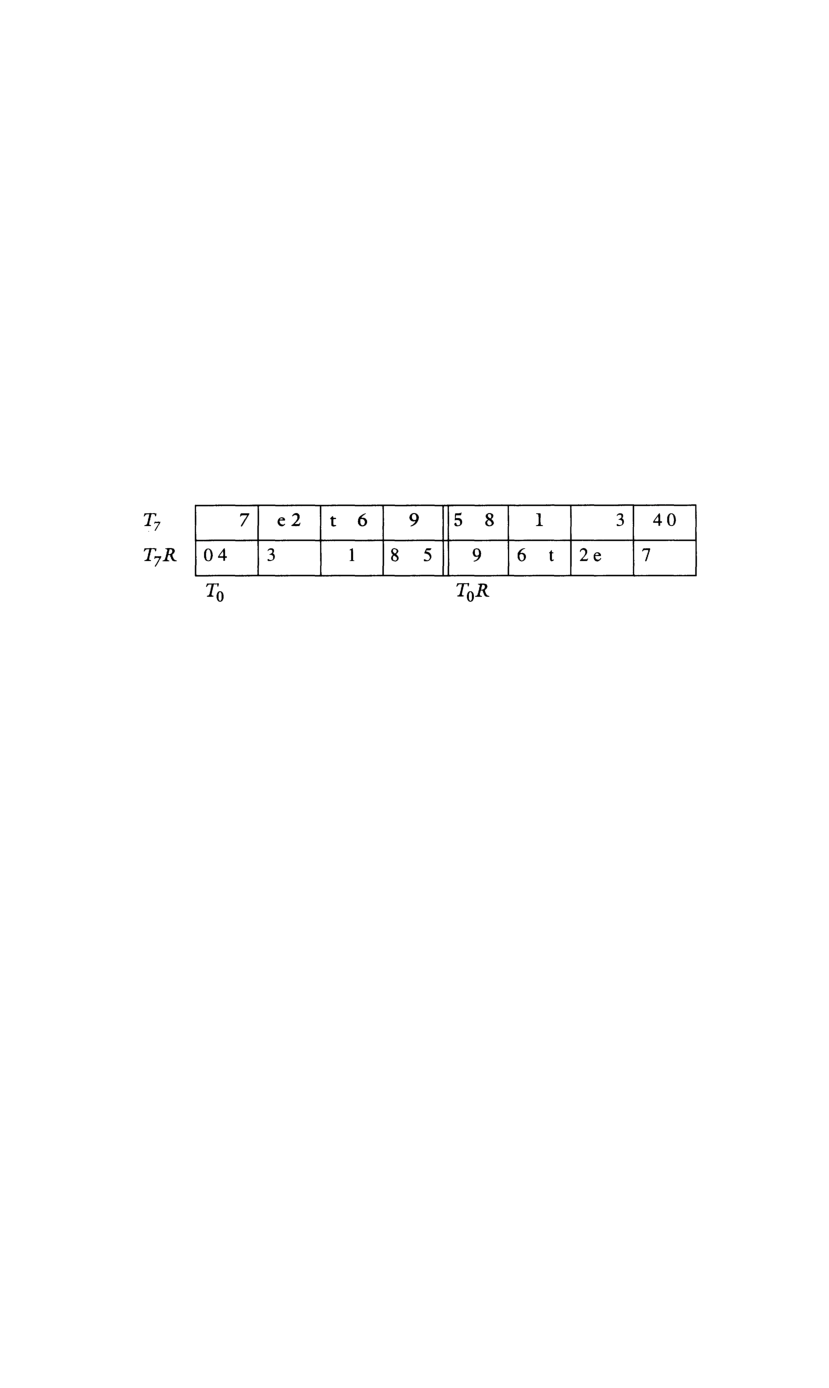
\includegraphics[width=\textwidth]{figures/scotto-array.pdf}
		\caption{Self-derived row in Scotto's \emph{Tetralogy}.}
	\end{figure}
\end{frame}

%------------------------------------------------------------------------
\begin{frame}
	\frametitle{Derivation in Scotto's \emph{Tetralogy}}
	We can fold the above matrix in order to obtain subsequent levels of derivation. The rows in the figure below are $\T_2(S), \R\T_2(S), \rho_6\R\T_2(S)$ and $\rho_6\T_2(S)$, where $\rho$ is the cyclical rotation operator.
	\begin{figure}
    	\centering
		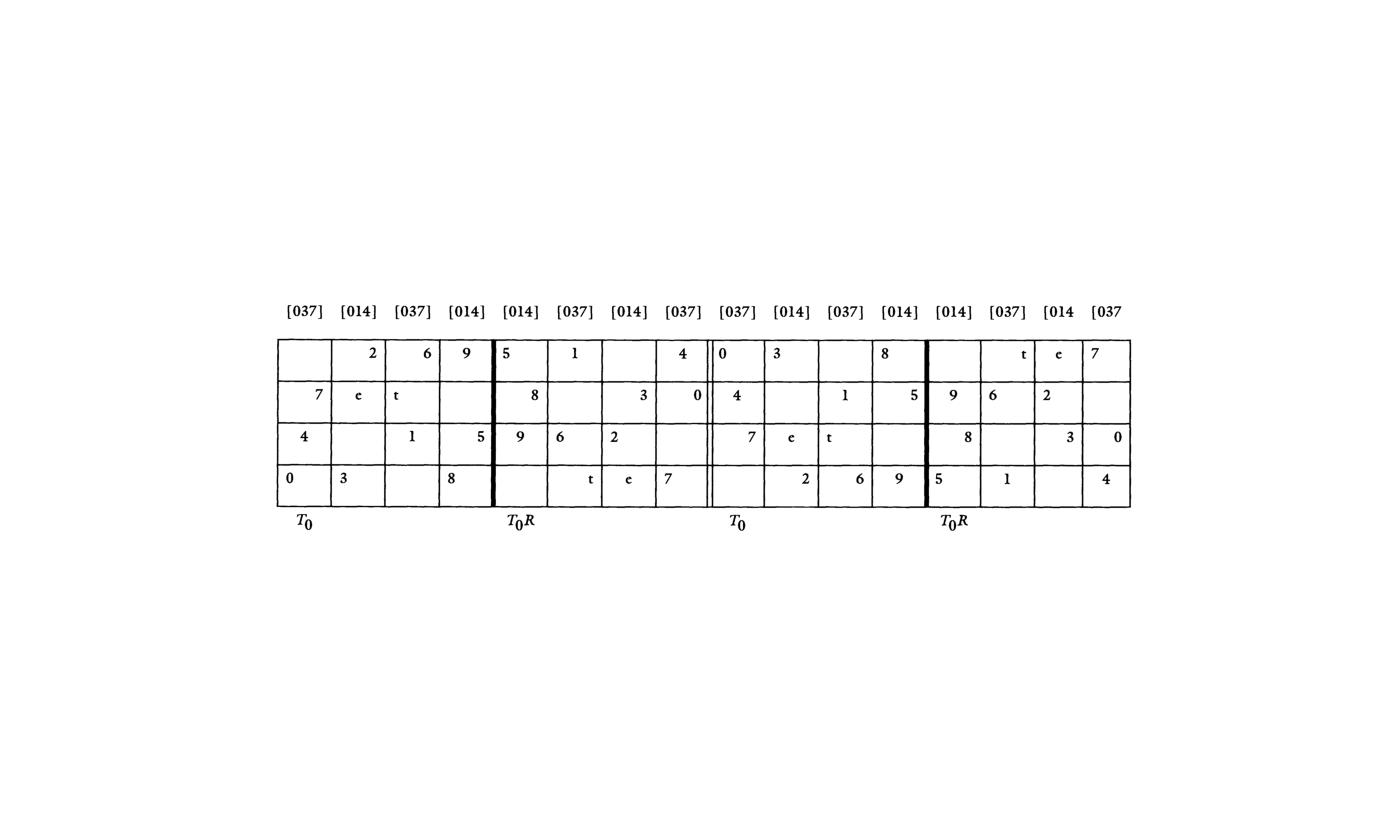
\includegraphics[width=3.2cm, angle=270]{figures/scotto-folded.pdf}
		\caption{Folded derivation in Scotto's \emph{Tetralogy}.}
	\end{figure}
\end{frame}

%------------------------------------------------------------------------
\begin{frame}
	\frametitle{Derivation in Scotto's \emph{Tetralogy}}
	\begin{figure}
    	\centering
		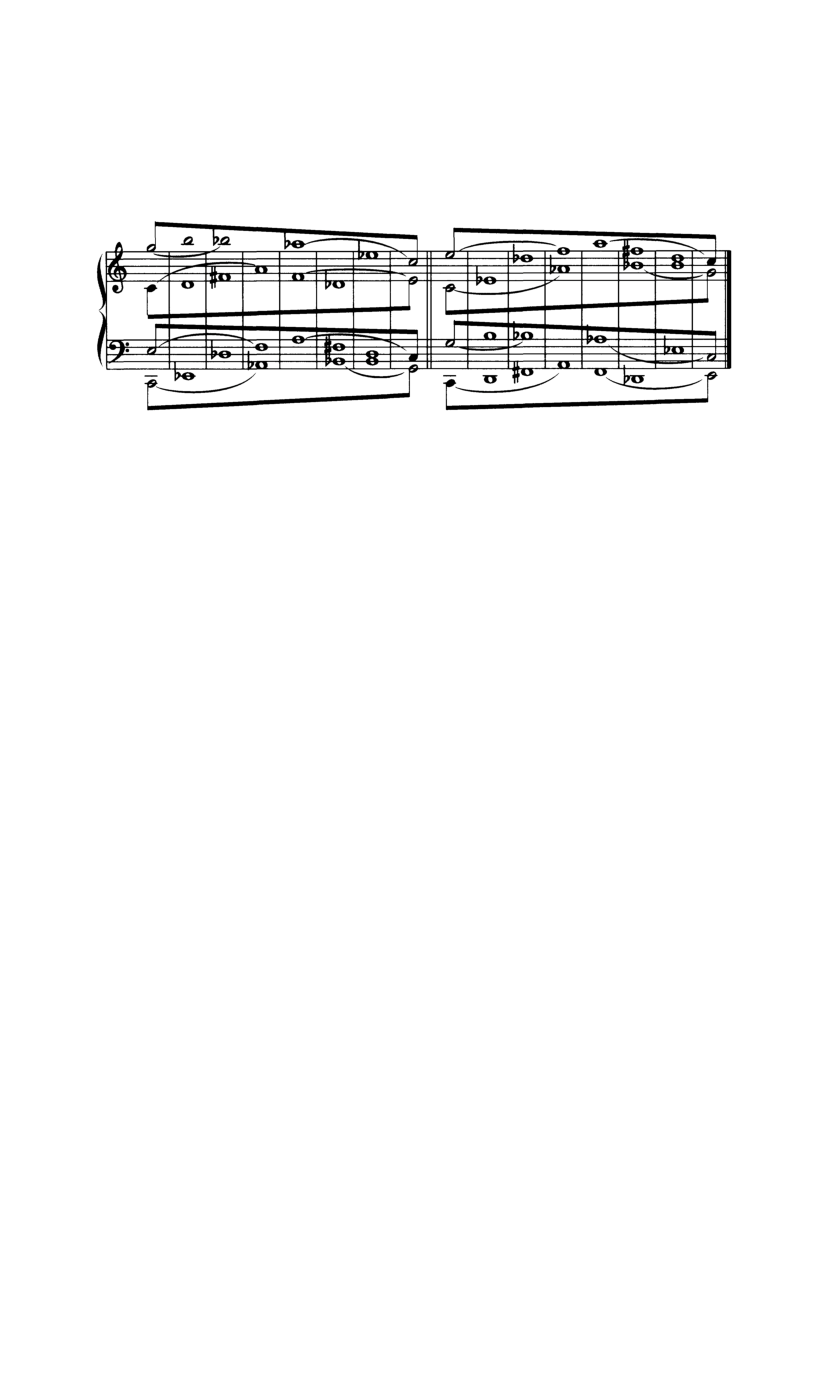
\includegraphics[width=\textwidth]{figures/scotto-schenker1.pdf}
		\caption{Schenkerian middle-ground structure in Scotto's \emph{Tetralogy}.}
	\end{figure}
\end{frame}

%------------------------------------------------------------------------
\begin{frame}
	\frametitle{Derivation in Scotto's \emph{Tetralogy}}
	\begin{figure}
    	\centering
    	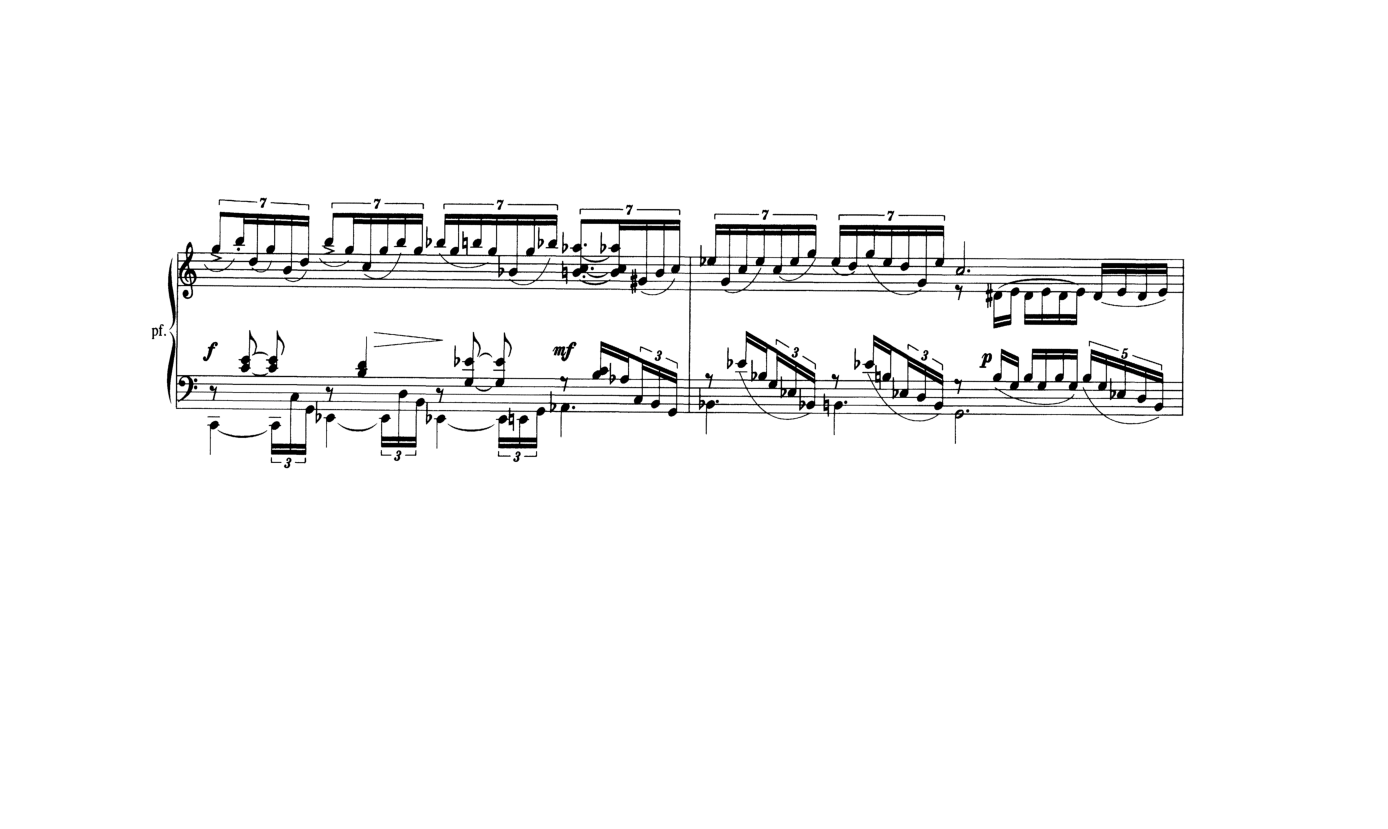
\includegraphics[width=3.2cm, angle=270]{figures/scotto-music1.pdf}
		\caption{Musical realization of the middle-ground in Scotto's \emph{Tetralogy}.}
	\end{figure}
\end{frame}

%------------------------------------------------------------------------
\begin{frame}
	\frametitle{Derivation in Scotto's \emph{Tetralogy}}
	The idea of prolongation in \emph{Tetralogy} extends beyond the foreground musical surface, and is applied as well to the middle-ground structure itself, effectively pushing it further into the background of the piece. 
	\begin{figure}
    	\centering
    	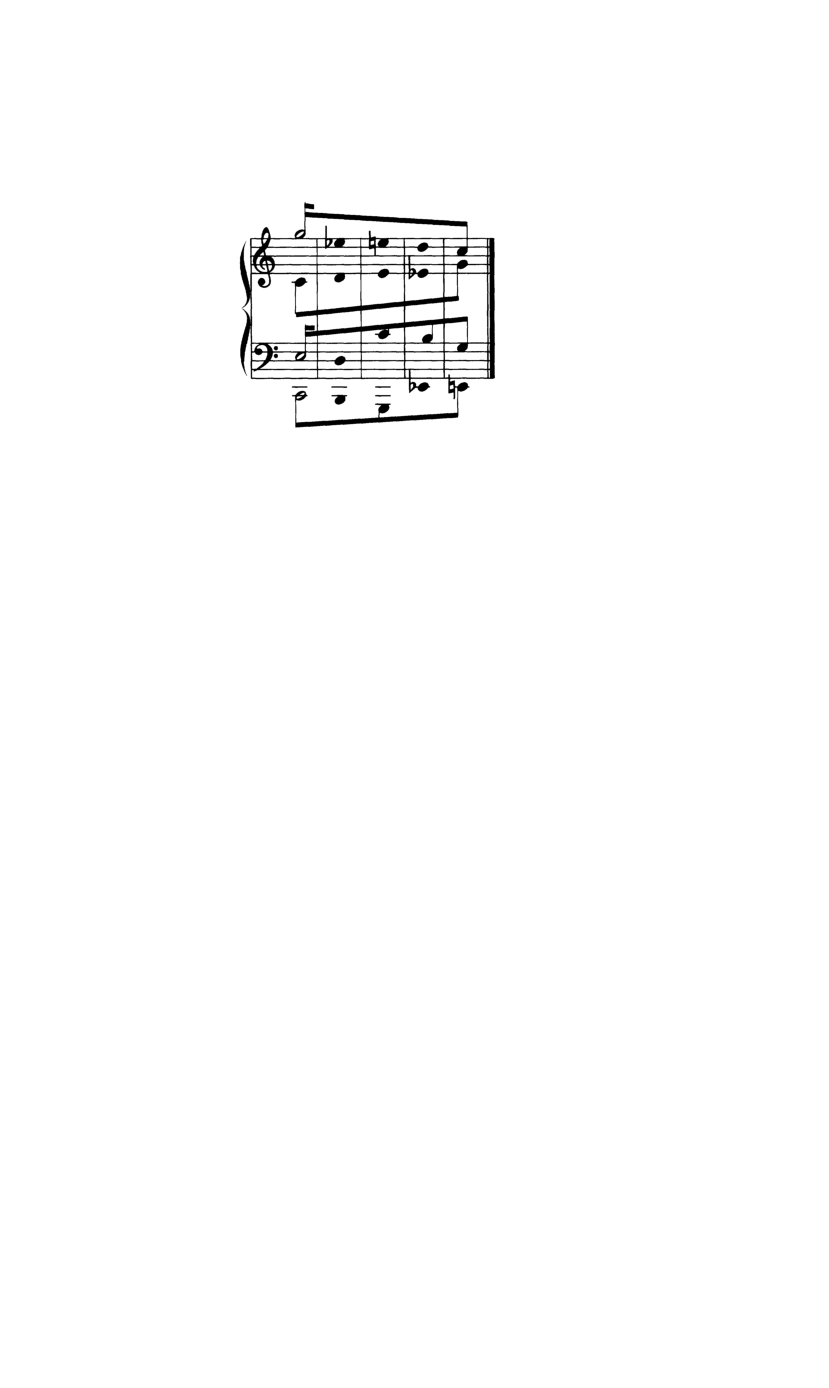
\includegraphics[width=5cm]{figures/scotto-schenker2.pdf}
    	\caption{Prolongation of the middle-ground structure in Scotto's \emph{Tetralogy}.}
	\end{figure}
\end{frame}

%------------------------------------------------------------------------
\begin{frame}
	\frametitle{Derivation in Scotto's \emph{Tetralogy}}
	\begin{figure}
    	\centering
    	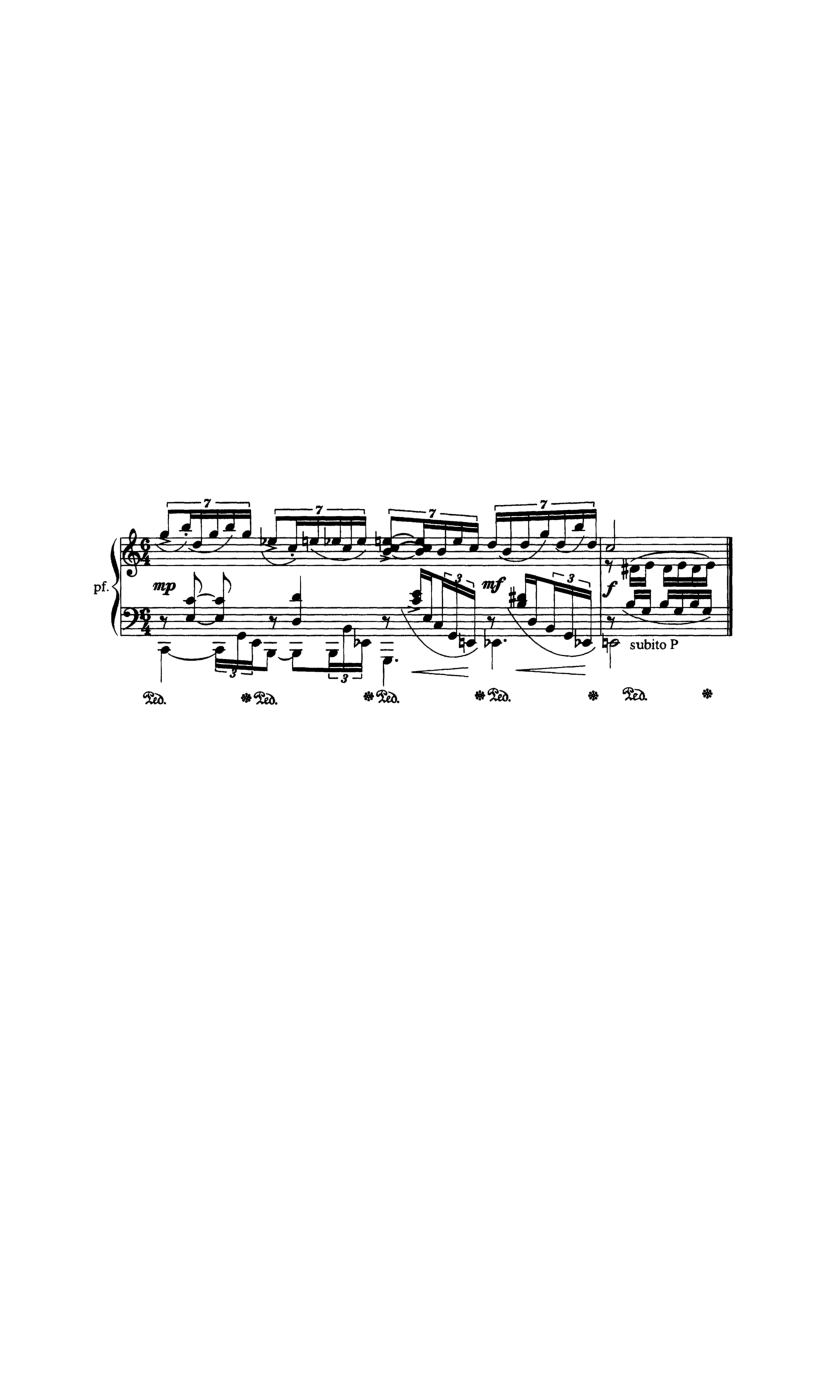
\includegraphics[width=\textwidth]{figures/scotto-music2.pdf}
    	\caption{Musical realization of the prolonged middle-ground in Scotto's \emph{Tetralogy}.}
	\end{figure}
\end{frame}
